% Vorlesung 1.9.19

\chapter{Grundlagen der Quantenmechanik}

\lcom{Dies ist das letzte Kapitel dieser Vorlesung. Vektor Algebra muss man für dieses Kapitel gut verstanden haben.}

\section{Axiome der Quantenmechanik}

\folie{Die Axiome der Quantenmechanik}
\begin{enumerate}[I)]
	\item Der Zustand wird beschrieben durch die Wellenfunktion $ \Psi $ bzw. den Zustandvektor $ |\Psi \rangle $\\
	$$ \Psi = \tx{ Wellenfunktion}$$
	$$ \vert\Psi\rangle = \tx{ Zustandsvektor, q.m. Zustand, Zustand}$$
	\item Einer Messbaren Eigenschaft ist ein hermitescher Operator $ \hat{A} $ zugeordnet, $ \hat{A} $ heißt Observable\\
	Impuls $\leftrightarrow$ $\vec{\hat p}$ = $\begin{pmatrix} \hat p_x \\ \hat p_y \\ \hat p_z \end{pmatrix}$\\
	Ort $\leftrightarrow\ \vec{\hat x}$\\
	Energie $\leftrightarrow\ \hat H$
	\item Der Erwartungswert eines Operators $ \hat{O} $ im Zustand $ |\Psi\rangle $ bzw. für die Wellenfunktion $ \Psi $ ist gegeben durch:
	 $ \langle \hat{ O \rangle} = (\Psi, \hat{O}, \Psi) \quad $ oder $ \quad \langle \hat O \rangle = \langle \Psi \vert \color{black!20!red}\hat O \color{black}\vert \color{black!30!green} \Psi \color{black}\rangle = \sum_n \overbrace{\color{black!30!green}p_n}^{\mathclap{\tx{Wahrscheinlichkeit}}} \underbrace{\color{black!20!red}a_n}_{\mathclap{\tx{Zahlen}}}$\\
	Wobei das erste $\langle \hat O \rangle$ das statistische Mittelwert bedeutet. \\
	\lcom{Diese aussage gilt für alle Operatoren, nicht nur Hermitesche.}
	\item Die Zeitentwicklung der Zustände bzw. Wellenfunktionen wird durch die Schrödinger-Gleichung beschrieben:\\
	$$ i\hbar \frac{\partial}{\partial t}\Psi = \hat{H}\Psi \quad \tx{bzw.} \quad i\hbar \frac{\partial}{\partial t} | \Psi \rangle = \hat{H}|\Psi \rangle$$
	\item Bei Messungen der Observablen $ \hat{A} $ für ein System im Zustand $ |\Psi \rangle $ bzw. der Wellenfunktion $ \Psi $ erhält man mit der Wahrscheinlichkeit $ p_n = |(\Psi_n, \Psi)|^2 $ bzw. $ p_n = |\langle \Psi_n | \Psi \rangle |^2 $ den Eigenwert $ a_n : $ der Zustand des Systems geht in die zugeordnete Eigenfunktion $ \Psi_n $ bzw. $ |\Psi_n\rangle $ über (Messprozess $ \rightarrow $ Kollaps der Wellenfunktion). \label{Axiom5}
\end{enumerate}
Außerdem gilt: Der Erwartungswert $ \langle \hat{A} \rangle $ der Observablen $ \hat{A} $ ist der Mittelwert der Messergebnisse $ a_n $ von sehr vielen (gleichen) Experimenten $ \langle \hat{A} \rangle = \sum_n p_n a_n $.

\section{Wellenfunktion, Operatoren, Zustände}

\subsection{Wellenfunktionen}

\subsubsection{Doppelspalt}

\folie{Interferenz/Einzel-Teilchen Experimente}\\
$$\vec{E}\tx{: relle, vektorielle Funktion um }\vec{r}\tx{ und }t$$
$$\Psi\tx{: komplexe, skalare Funktion von } \vec{r} \tx{ und }t$$

\subsubsection{Interpretation der Wellenfunktion}

$|\Psi(\vec{r},t)|^2$ ist die Wahrscheinlichkeit dafür ein Teilchen zur Zeit $t$ am Ort $\vec{r}$ zu finden.\\

\subsubsection{$\Rightarrow$ Normierung}

Gesamtwahrscheinlichkeit muß 1 sein. $\Rightarrow\ \int \Psi^*(\vec{r},t) \Psi(\vec{r},t) \dd \vec{r} = 1$ wobei $\Psi^*$ das komplex konjugierte ist.

\subsection{Operatoren}

\lcom{Die mathematische Definition ist fürchterlich einfach.}

\subsubsection{Mathematische Definition}

$$\Psi' = \hat O \Psi \qquad |\Psi'\rangle = \hat O | \Psi \rangle$$

\subsubsection{Anschauliche Definition}

Ein Operator verändert einen Zustand.\\
\bei
$$\Psi'(\vec{r},t) = C e^{\frac{i}{\hbar} (\vec{p} \cdot \vec{r} - Et)}$$
\begin{itemize}
	\item $\hat O = (5 + 3i) \qquad \Psi'(\vec{r}, t) = (5 + 3i) \Psi(\vec{r},t) = (5 +3i)C e^{\frac{i}{\hbar}(\vec{p}\vec{r}- Et)}$
	\item $\hat O = \prt{}{t} \qquad \Psi'(\vec{r}, t) = \prt{}{t}\Psi(\vec{r},t) = -C\frac{i}{\hbar}E e^{\frac{i}{\hbar}(\vec{p}\vec{r}- Et)}$
	\item $\hat O = \prt{}{x} \qquad \Psi'(\vec{r}, t) = \prt{}{x} \Psi(\vec{r},t) = C\frac{i}{\hbar}p_x e^{\frac{i}{\hbar}(\vec{p}\vec{r}- Et)}$
	\item $\hat O = \tx{Zeitumkehroperator}:\ \hat T \qquad \Psi'(\vec{r}, t) = \hat T \Psi(\vec{r},t) = \Psi(\vec{r},-t)$
\end{itemize}
\subsection{Hilbert-Raum (Ultrakompakt)}
Frage: Was ist der Unterschied bzw. Zusammenhang zwischen $\Psi$ und $|\Psi\rangle$???\\
Antwort:
\rbox{$\Psi(\vec{r},t)$ ist die Wellenfunktion des Zustandes $|\Psi(\vec{r},t)\rangle$ in der Ortsdarstellung.}
\subsubsection{Vektorraum}
$$\vec{v}(t) = \sum_k c_k (t) \vec{e}_k$$
$\custo{\rightarrow}{\tx{Vektor}}{\ |\Psi\rangle}$ = $\custo{\rightarrow}{\tx{Koordinaten}}{\ \Psi}$ und $\custo{\rightarrow}{\tx{Basisvektoren}}{\tx{Darstellung}}$ (Koordinatensystem) 

\subsubsection{Reihenentwicklung von Funktionen, Funktionen als Vektorraum}

\begin{equation*}
f(x) = \sum_{k} c_k g_k(x) \qquad \tx{diskreten}
\end{equation*}
\begin{equation*}
\tx{Funktion } = \tx{ Entwicklungskoeffizienten } \& \tx{ Funktionenbasis}
\end{equation*}
\begin{enumerate}[(1)]
	\item endlich diskret
	\begin{equation*}
	f(x) = \sum_{k=0}^{N} c_k g_k(x)
	\end{equation*}
	\item unendlich diskret
	\begin{equation*}
	f(x) = \sum_{k=0}^{\infty} c_k g_k(x)
	\end{equation*}
	\item kontinuierlich
	\begin{equation*}
	f(x) = \int c(k) g(k,x) \dd k
	\end{equation*}
	\item diskret + kontinuierlich
	\begin{equation*}
	f(x) = \sum_{k} c_k g_k(x) + \int c(k) g(k,x) \dd k
	\end{equation*}
\end{enumerate}
\emph{Beispiele:}
\begin{itemize}
	\item Fourier-Reihe: unendlich diskret
	\begin{equation*}
	f(x) = \frac{a_0}{2} + \sum_n a_n \cos(n \omega_0 t) + b_n \sin(n \omega_0 t)
	\end{equation*}
	\item Fourier-Integral/Transformation: kontinuierlich
	\begin{equation*}
	f(x) = \int F(\omega) e^{-i \omega t} \dd \omega
	\end{equation*}
	$ e^{-i \omega t} : $ Basisfunktionen\\
	$ F(\omega) : $ Entwicklungskoeffizienten
	\item Kugelflächenfunktionen:
	\begin{equation*}
	f(0,1) = \sum_{l = 0} \sum_{m = -l}^{l} c_{lm} Y_{m}^{l}(0,1)
	\end{equation*}
	\item Taylor-Reihe:
	\begin{equation*}
	f(x) = \sum_n \frac{1}{n !} f^{(n)} (0) x^n
	\end{equation*}
	\item Legendre-Polynome:
	\begin{equation*}
	f(x) = \sum_n c_n P_n(x)
	\end{equation*}
\end{itemize}
\lcom{Sehr allgemeines Konzept, es gibt viele Beispiele wie Hermitesche Polynome.}

\subsubsection{Hilbertraum}

Ähnlich wie ein Vektorraum, nur mit Funktionen als Basis.
\begin{equation*}
\tx{Funktionsbasis } + \tx{ gewisse Eigenschaften}
\end{equation*}

\subsubsection{Bracket-Notation}

\begin{equation*}
|\custo{\leftarrow}{\quad}{\mathclap{\tx{Freiraum}}} \rangle
\end{equation*}
\begin{equation*}
|\Psi\rangle , |\vec{r}, t \rangle , | \Psi, t \rangle , | n \rangle , | E \rangle , | \dots \rangle
\end{equation*}
\lcom{die Bracket können vieles bedeuten wie zum Beispiel $f(x)$ kann alle möglichen Funktionen darstellen.}

\subsection{Zustand Darstellung und Wellenfunktion}

\begin{alignat*}{3}
&|\Psi\rangle = &&\Psi \qquad \tx{und} &&| n\rangle\\
&\tx{Zustand}\quad &&\tx{Wellenfunktion}\quad &&\tx{Darstellung}\\
&\vec{v} = &&\tx{Koordinaten} &&\tx{Basisvektoren}
\end{alignat*}

% hier ein bisschen misst der so gesagt wurde und dann aus dem kontext genommen wurde
\begin{comment}
\chapter{Der Liebe Gott}
\section{Verliebt sein}
\subsection{wer darf wo rumfumeln}
rumfumeln ist nicht unabhängig
\subsection{was gehört zu wem}
\section{Gender-Theorie}
es gibt unendliche viele Wahrscheinlichkeiten und Zuordnungen (von Gendern)
\section{Der Satz von Stinson}
\end{comment}

% Vorlesung 15.01.18


% andrez:
% 1.15.19
%
%\bbb{Wiederholung}{QM}
%
\noindent
QM-Zustand: $ \widehat = $ Zustandsfunktion $ |\Psi , t \rangle $\\
Darstellung: $ \widehat = $ gewählter Basisfunktionensatz $ | n \rangle $\\
Wellenfunktion: $ \Psi (\vec{r},t) \widehat = $ Entwicklungskoeffizienten in Ortsdarstellung\\
Darstellungswechsel: $ \widehat = $ Koordinatentransformation/Basiswechsel\\
\bei 
\begin{itemize} 
	\item Ortsdarstellung: Basis sind die Ortseigenfunktionen $|\vec{r}\rangle$
	$$\vec{\hat r} | \vec{r} \rangle = \vec{r}| \vec{r}\rangle$$
	$$\Rightarrow |\Psi, t\rangle =\int \underbrace{\Psi(\vec{r},t)}_{\mathclap{\tx{Wellenfkt. in Ortsdarstellung}}}|\vec{r}\rangle \dif\vec{r}$$
	\item Impulsdarstellung: Basis sind die Impulseigenfunktion $|\vec{p}\rangle$
	$$\vec{\hat p} |\vec{p} \rangle = \vec{p} | \vec{p}\rangle$$
	$$\Rightarrow |\Psi, t \rangle =\int \underbrace{\Psi(\vec{p},t)}_{\mathclap{\tx{Wellenfkt. in Impulsdarstellung}}}|\vec{p}\rangle \dd \vec{p}$$
	\item Energie- (Spektral-) Darstellung: Basis sind Energieeigenfunktionen $|E_n \rangle$
	$$\hat \ham| E_n\rangle = E_n|E_n\rangle$$
	$$\Rightarrow |\Psi,t\rangle =\sum_k \underbrace{C_k (t)}_{\substack{ \\[5pt] \mathclap{\tx{Wellenfkt. in der Energiedarstellung}}}} |E_n\rangle$$
\end{itemize}

\subsection{Analogie zwischen Vektor- und Hilbertraum}
$$\vec{v}(t) = \sum_k C_k (t) \vec{e}_k \qquad \leftrightarrow \qquad |\Psi,t\rangle = \sum_n C_n (t) |n\rangle \quad \tx{oder} \quad |\Psi,t\rangle = \int C(n,t)|n\rangle\dif n$$
\folie{Analogie zwischen Vektor- und Hilbertraum}

\subsubsection{Vektoroperator}
$$\vec{p} = \begin{pmatrix} p_x \\ p_y \\ p_z \end{pmatrix} \hat = \mathop{} \vec{\hat p} = \begin{pmatrix}\hat p_x \\ \hat p_y \\ \hat p_z \end{pmatrix}$$
\lcom{Wir brauchen alle drei Zahlen um die Bewegung des Teilchens zu beschreiben.}
\section{Nicht relativistische QM und Schrödingergleichung}
\subsection{Zustand und Bewegung eines Teilchens}

klassisch:
\begin{description}
	\item[Zustand] $\vec{v}(t), \vec{p}, t$
	\item[Messgrößen] können ausgedrückt werden als Funktionen um $\vec{v}(t), \vec{p}(t),t, \dots$
	\item[Bewegung] Hamiltonfunktion $\ham(\vec{r},\vec{p}) = E$
\end{description}
QM, in der Sprache der Wellenfunktionen in der Ortsdarstellung
\begin{description}
	\item[Zustand] Wellenfunktion $\Psi(\vec{r},t)$
	\item[Messgrößen] Eigenwert $a_k$ der Observable $\hat A$ mit einer Wahrscheinlichkeit $p_k = |(\Psi_k, \Psi)|^2$
	\item[Bewegung] Hamiltonoperator $\hat \ham(\vec{\hat r},\vec{\hat p})$
	$$i \hbar \prt{}{t} \Psi(\vec{r}, t) = \hat \ham \Psi(\vec{r}, t)$$
\end{description}
QM in der Sprache der Zustandsfunktionen
\begin{description}
	\item[Zustand] $|\Psi,t\rangle$
	\item[Messgrößen] Eigenwert $a_k$ der Observable $\hat A$ mit einer Wahrscheinlichkeit $p_k = |\langle\Psi_k | \Psi\rangle|^2$
	\item[Bewegung] $$i \hbar \prt{}{t} | \Psi(\vec{r}, t) \rangle = \hat \ham |\Psi,t\rangle$$
\end{description}
$ \rmbox{\vec{F} = m \vec{a}} $

\subsubsection{Wichtige Darstellung}

\begin{itemize}
	\item $t$ ist ein Parameter
	\item $\vec{r}$ in $\Psi(\vec{r},t)$ hängt nicht implizit selber von $t$ ab.
	\item $\vec{r}$ in $\Psi(\vec{r},t)$ ist \color{red} NICHT \color{black} der Ort des Teilchens \mau\\
	Der Ort der Teilchens ergibt sich aus Axiom V)
	$$p(\vec{r}) = |(\Psi_{\vec{r}}|\Psi)|^2 = |\Psi(\vec{r},t)|^2$$
	\item $\Psi(\vec{r},t)$ hängt \color{red} NUR \color{black} von $\vec{r}$ und $t$ ab, \color{red} NICHT \color{black} von z.B. $\vec{p}, E, \dots$\\
	Der Impuls des Teilchens ergibt sich aus Axiom \ref{Axiom5}
	$$p(\vec{p}) = |(\Psi_p | \Psi)|^2 = \cancel{| \Psi(p,t)|^2}$$
\end{itemize}

%markus:
\subsection{,,Herleitung`` der Schrödingergleichung (SGL)}

Wir betrachten ein freies Teilchen $ \widehat{=} $ Ebene Welle $ \quad \Psi(\vec{r},t) = C e^{\frac{i}{\hbar} (\vec{p} \cdot \vec{r} - E t)} $

\subsubsection{Ortsoperator}

\begin{equation*}
\hat{\vec{r}} \Psi = \vec{r} \Psi \quad \tx{ nach Konst}
\end{equation*}
\lcom{Dies geht, da der Ortsoperator auf $ \Psi $ angewendet gleich $ \vec{r} \Psi $ ist.}

\subsubsection{Impulsoperator}

\begin{equation*}
\hat{\vec{p}} \Psi = \vec{p} \Psi
\end{equation*}
Beobachte: $ \prt{}{x} \Psi = \frac{i}{\hbar} p_x \Psi \quad \Rightarrow \quad \vabla \Psi = \frac{i}{\hbar} \vec{p} \Psi $
\begin{equation*}
\Rightarrow \quad \rmbox{\hat{\vec{p}} = - i \hbar \vabla} \quad \tx{ Impulsoperator in der Ortsdarstellung}
\end{equation*}

\subsubsection{Schrödinger-Gleichung}

\begin{equation*}
\hat{E} \Psi = E \Psi
\end{equation*}
Beobachte: $ \prt{}{t} \Psi = - \frac{i}{\hbar} E \Psi $
\begin{equation*}
\Rightarrow \quad \rmbox{\hat{E} = i \hbar \prt{}{t}}
\end{equation*}
Neben klassischer Gleichung $ \ham(\vec{r},\vec{p}) = E $, und ersetzen durch Operatoren
\begin{equation*}
\rmbox{i \hbar \prt{}{t} \Psi(\vec{r},t) = \hat{\ham}(\hat{\vec{r}}, \hat{\vec{p}}) \Psi(\vec{r},t)}
\end{equation*}
$ \Rightarrow $ Verallgemeinerung: Zeitabhängige Schrödinger-Gleichung
\frbox{Zeitabhängige Schrödinger-Gleichung}{
\begin{equation*}
i \hbar \prt{}{t} |\Psi,t\rangle = \hat{\ham} (\hat{\vec{r}}, \hat{\vec{p}}) |\Psi,t\rangle
\end{equation*}
}

\subsection{Freies Teilchen in Ortsdarstellung}

klassisch:
\begin{equation*}
\ham (\vec{r}, \vec{p}) = \frac{\vec{p^2}}{2 m}
\end{equation*}
quantenmechanisch:
\begin{equation*}
\hat{\ham} = \frac{\hat{\vec{p}}^2}{2 m} = - \frac{\hbar^2}{2 m} \vabla^2 \qquad (\vabla^2 = \prt{^2}{x^2} + \prt{^2}{y^2} + \prt{^2}{z^2} = \Delta)
\end{equation*}
da $ \hat{\vec{p}} = - i \hbar \vabla $\\[5pt]
Schrödingergleichung:
\begin{equation*}
i \hbar \prt{}{t} \Psi(\vec{r},t) = - \frac{\hbar^2}{2 m} \vabla^2 \Psi(\vec{r},t)
\end{equation*}
\textbf{Lösung:}
\begin{enumerate}[i)]
	\item Lösungsansatz:
	\begin{equation*}
	\Psi(\vec{r},t) = Ce^{\frac{i}{\hbar} (\vec{p} \cdot \vec{r} - E t)}
	\end{equation*}
	\item 1. Seite der Schrödinger-Gleichung: $ \quad i \hbar \prt{}{t} \Psi = E \Psi $
	\item 2. Seite der Schrödinger-Gleichung: $ \quad -\frac{\hbar^2}{2 m} \left(\frac{i}{\hbar} \vec{p}\right)^2 \Psi = \frac{\vec{p}^2}{2 m} \Psi $
	\begin{equation*}
	\Rightarrow \quad E \cancel{\Psi} = \frac{\vec{p}^2}{2 m} \cancel{\Psi}
	\end{equation*}
	\begin{equation*}
	\rmbox{E = \frac{\vec{p}^2}{2 m}} \quad \checkmark \qquad \Rightarrow \quad \Psi(\vec{r},t) = C e^{\frac{i}{\hbar} (\vec{p} \cdot \vec{r} - E t)}
	\end{equation*}
\end{enumerate}

\subsection{Teilchen im Potential in Ortsdarstellung}

klassisch:
\begin{equation*}
\ham(\vec{r},\vec{p}) = \frac{\vec{p}^2}{2 m} + V(\vec{r})
\end{equation*}
quantenmechanisch:
\begin{equation*}
\hat{\ham} = - \frac{\hbar^2}{2 m} \vabla^2 + V(\vec{r})
\end{equation*}
Schrödinger-Gleichung:
\begin{equation*}
i \hbar \prt{}{t} \Psi(\vec{r},t) = \left(- \frac{\hbar^2}{2 m} \vabla^2 + V(\vec{r})\right) \Psi(\vec{r},t)
\end{equation*}
\emph{Bemerkung:}
\begin{itemize}
	\item ebene Wellen sind \textbf{keine Lösung} dieser SGL
	\begin{equation*}
	\Psi = \tx{ ebene Welle} \quad \Rightarrow \quad E = \frac{\vec{p}^2}{2 m} + V(\vec{r}) \qquad \tx{weil in Ortsdarstellung gilt: } \quad \hat{\vec{r}} \Psi = \vec{r} \Psi 
	\end{equation*}
	\LARGE{\lightning} \normalsize $ E \neq \const : \quad E(\vec{r}) $\\
	Wir wissen aber $ E $ ist nicht vom Ort abhängig sondern eine Konstante.\\
	Hier ist der Lösungsansatz also Falsch. \LARGE{\lightning} \normalsize
\end{itemize}

\subsection{Zeitunabhängige SGL}

Für explizit nicht von der Zeit abhängiger Hamiltonoperatoren läßt sich die SGL allgemein lösen:\\[5pt]
Ansatz:
\begin{equation*}
|\Psi,t\rangle = f(t) |\Psi,0\rangle
\end{equation*}
$ \Rightarrow $ in zeitabhängige SGL einsetzen $ \Rightarrow $ Gleichung separieren $ \Rightarrow $ zwei Gleichungen für die zwei separierten Bruchstücke
\begin{enumerate}[(1)]
	\item eine Lösung stellt sich als eindeutig heraus
	$$ f(t) = e^{-\frac{i}{\hbar} Et} $$
	\item$ \phantom{0} $\\[-30pt]
	\frbox{Zeitunabhängige Schrödinger-Gleichung}{
	\begin{equation*}
	\hat{\ham} |\Psi,0\rangle = E |\Psi,0\rangle
	\end{equation*}
	}
\end{enumerate}
\textbf{Feststellung 1:}
\begin{equation*}
\rmbox{\tx{Das ist eine Eigenwertgleichung zum Hamiltonoperator}}
\end{equation*}
\begin{equation*}
\begin{array}{l|l}
	\tx{diskret} & \tx{kontinuierlich}\\
	\hline\\[-5pt]
	\hat{\ham} |n\rangle = E_n |n\rangle & \hat{\ham} |n\rangle = E(n) |n\rangle\\
\end{array}
\end{equation*}
$ n $ abzählbar\\
\textbf{Energiezustände} $ |n\rangle $\\
Energie-Eigenwerte $ E_n $ bzw. $ E(n) $\\[5pt]
\textbf{Feststellung 2}
\begin{center}
	\begin{minipage}{.65\linewidth}
			\rbox{Die Lösungen der zeitunabhängigen SGL sind die \\ \textbf{stationären Zustände} des Quantensystems}
	\end{minipage}
\end{center}
Zeitabhängigkeit stationärer Zustände
\begin{equation*}
|n,t\rangle = e^{-\frac{i}{\hbar} E_n t} |n\rangle
\end{equation*}
Zeitabhängigkeit von Zeitunabhängigen Erwartungswerten in stationären Zuständen
\begin{equation*}
\langle \hat{O} \rangle (t) \equiv \langle n | e^{\frac{i}{\hbar} E_n t} \hat{O} e^{-\frac{i}{\hbar} E_n t} |n \rangle = \langle n | \hat{O} | n \rangle = \const
\end{equation*}
Damit gilt auch $ \langle n , t | n , t \rangle = \langle e^{\frac{i}{\hbar} E_n t} e^{-\frac{i}{\hbar} E_n t} | n \rangle = \langle n | n \rangle = 1 = \const $ Somit ist der Begriff ,,stationärer Zustand`` gerechtfertigt.\\[5pt]
\textbf{Feststellung 3}\\
F1 ist äquivalent zu F2\\[10pt]

% Vorlesung 16.01.18

%andrez:
\bbb{Wiederholung}{Ansatz: $$|\Psi,t\rangle = f(t)|\Psi,0\rangle$$
	1) $f(t) = e^{-\frac{i}{\hbar} Et}$\\
	2) $ \hat \ham |\Psi,0\rangle = E|\Psi,0\rangle$\\
	Festellung 2:
	$$\langle \hat O \rangle(t) = \tx{mit unabhängig für stationäre zustände}$$}

\subsection{Zusammenfassung}

\begin{description}
	\item[Zustand, Wellenfunktion, Darstellung] $|\Psi\rangle = \sum_k \Psi_k|k\rangle$ oder $|\Psi\rangle = \int \Psi(k)|k\rangle \dif k$
	\item[Operatoren] $\Psi' = \hat O \Psi, \quad |\Psi'\rangle = \hat O| \Psi\rangle$
	\item[Messung] Axiom \ref{Axiom5}
	\item[Bewegung] const. $i\hbar \prt{}{t}|\Psi,t\rangle = \hat \ham |\Psi,t\rangle$
	$$\tx{ plus } \quad \prt{}{t}\hat \ham = 0 \quad E|\Psi\rangle = \hat \ham|\Psi\rangle, \quad |\Psi,t\rangle = e^{\frac{i}{\hbar}Et}|\Psi\rangle$$
\end{description}

\section{Stern-Gerlach Experiment und Elektronen-Spin (1922 - 25)}

Ziel: Messung des magnetischen Moments $\vec{\mu}$ von Atomen
$$\vec{\tau} = \vec{\mu} \times \vec{B}$$
\lcom{In einem inhmogenen Magnetfeld gibt es einen Feldgradienten undgleich null und damit eine Faraday-Kraft:}\\
Faraday Kraft $\vec{F} = \vec{\nabla}(\vec{\mu}\cdot\vec{B})$\\[5pt]
\begin{minipage}{.75\linewidth}
	\textbf{Vorbereitung:}\\[5pt]
	$\vec{L} = \vec{r} \times \vec{p}$\\
	$\vec{\mu} = IA \vec{n}$
	$$\Rightarrow \quad \rmbox{\vec{\mu} = \frac{q}{2m}\vec{L}}\quad \tx{Klassisch}$$
\end{minipage}%
\begin{minipage}{.25\linewidth}
	\flushright
	%t1 :
	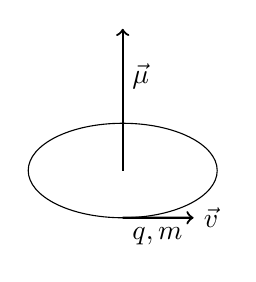
\begin{tikzpicture}[scale=.6]
		\draw[thick, ->] (0,0) -- (0,3);
		\draw (0,0) ellipse(2cm and 1cm);
		\coordinate (a) at (0,-1);
		\node[right] at (0,2) {$\vec{\mu}$};
		\node[anchor=north west] at (a) {$q,m$};
		\draw[thick,->] (a) -- (1.5,-1) node[right] {$\vec{v}$};
	\end{tikzpicture}
\end{minipage}%

\subsubsection{Aufbau und Durchführung}

Klassische Erwartung % $$\vec{\mu}$$: vermutlich nichts:
$$\vec{F} = \vec{\nabla}(\vec{\mu} \cdot \vec{B}) = \underbrace{\mu_z}_{\mathclap{\color{red}\tx{wird gemessen}}} \prt{B}{z} \vec{e}_z$$
Ofen $\Rightarrow$ statische Verteilung der Richtungen des $\vec{\mu}$'s der Atome

\subsubsection{Experiment}

\folie{The Spin, A Quantum Magnet (video)}\\[10pt]
\versuch{Magnetische Dipole durch inhomogenes Feld}
$ \Rightarrow $ nur zwei arten von Dipolen werden gemessen $ \pm p_z $, da nur $ p_z $ gemessen wird.\\
So als würden nur Dipole mit zwei verschiedenen Richtungen in das inhomogene Magnetfeld eintreten. Wir wissen aber, dass die eintretenden Dipole in \textbf{alle Richtungen} zeigen.\\[10pt]
Schlussfolgerungen:
\begin{enumerate}[1)]
	\item Das Elektron trägt neben der Ladung zusätzlich ein magnetisches Moment $ \vec{\mu}_e $.
	\begin{equation*}
	\Rightarrow \quad \tx{ ,,Eigendrehimpuls`` oder auch Spin } \quad \vec{S}
	\end{equation*}
	\item Es existiert eine räumliche Quantisierung des magnetischen Moments.
	\item $ \Rightarrow $ das magnetische Moment hat zwei ,,Einstellungen``\\
	$ \Rightarrow $ $ S = \frac{1}{2} $
	\item Zusammenhang zwischen $ \vec{\mu}_e $ und $ \vec{S} $ ist ca. 2-mal größer als klassisch erwartet.
	\begin{equation*}
	\mu_z = - g \mu_B \frac{S_z}{\hbar} \qquad g = 2 \qquad S_z = \pm \frac{1}{2}
	\end{equation*}
	\lcom{Das Minus Zeichen kommt daher, dass $ \mu_B $ eine positive Naturkonstante ist und die Ladung eines Elektrons $ e $ negativ.}
	\item Zum Elektronenspin gibt es \textbf{kein} klassisches Analogon.
	$ \Rightarrow $ es gibt z.B. kein $ \Psi(\vec{r},t) $ also keinen Spin in der Ortsdarstellung.
\end{enumerate}
\emph{Bemerkung:}
\begin{itemize}
	\item $ \vec{S} $ ist für uns über $ \vec{\mu} $ messbar $ \rightarrow  \left\{\begin{array}{l}
	\tx{Observable} \\ \tx{3D Vektor}
	\end{array}\right. $
\end{itemize}

\section{Zustand, Wellenfunktion und Messprozess}

\subsection{Elektronenspin}

Zustandsfunktion
\begin{equation*}
|\Psi\rangle = \tx{ Linearkombi. von Wellenfunktionen mal Basisfunktionen } = \sum_n c_n |n\rangle
\end{equation*}
(Die Wellenfunktionen sind hier die Entwicklungskoeffizienten)
\begin{equation*}
|\Psi \rangle = \alpha |\uparrow \: \rangle + \beta |\downarrow \: \rangle
\end{equation*}
Beim Elektronenspin haben wir eine 2-dimensionalen Hilbertraum \mau\\[5pt]
$ \alpha, \beta : $ komplexe zahlen\\
$ \alpha^2 + \beta^2 = 1 : $ Normierung\\[5pt]
\lcom{Die Ortsfunktion ,,lebt`` in einem Unendlich-dimensionalen Hilbertraum!}\\[5pt]
\emph{Bemerkung:}
\begin{itemize}
	\item Analogie 2-dim Vektorraum $ \vec{v} = x \vec{e}_x +  \vec{e}_y = x_1 \vec{r}_1 + x_2 \vec{e}_2 = \dots $
	\item Wir haben ,,unbemerkt`` eine Quantisierungsachse festgelegt (bei uns bis jetzt die $ z $-Achse)\\
	\lcom{Dies bedeutet es gibt kein Experiment bei dem man gleichzeitig mehrere Komponenten von $ \vec{\mu} $ misst. Man könnte zuerst die $ z $-Richtung messen und danach versuche die $ x $-Richtung zu messen, aber nicht gleichzeitig.}
	\begin{equation*}
	\Rightarrow \quad \begin{array}{l}
	| \uparrow \: \rangle \\ | \downarrow \: \rangle
	\end{array} \quad \tx{ sind mit der Richtung der Quantisierungsachse verknüpft !}
	\end{equation*}
	\item  Erinnerung:
	\begin{equation*}
	|\Psi\rangle = \alpha | \uparrow \: \rangle + \beta | \downarrow \: \rangle \qquad \alpha = \langle \: \uparrow | \Psi \rangle \qquad \beta = \langle \: \downarrow | \Psi \rangle
	\end{equation*}
	%%% (1)
	Analogie Vektorraum:
	$$ \vec{v} = \alpha \vec{e}_1 + \beta \vec{e}_2 \quad \Rightarrow \quad \alpha = \vec{e}_1^\top \cdot \vec{v} \qquad \beta = \vec{e}_2^\top \cdot \vec{v} $$
\end{itemize}
\textbf{Wellenfunktion:}\\[5pt]
\begin{minipage}{.6\linewidth}
	Wie schauen $ | \uparrow \: \rangle $ und $ | \downarrow \: \rangle $ aus?\\
	$ \Rightarrow $ keine Ahnung\\[5pt]
	Was wir nur wissen ist wie Operatoren auf sie wirken
	\begin{equation*}
	\hat{S}_x, \hat{S}_y, \hat{S}_z , (\vec{S})^2
	\end{equation*}
	\begin{align*}
	\hat{S}_z \ | \uparrow \: \rangle &= + \frac{1}{2} \ | \uparrow \: \rangle \\
	\hat{S}_z \ | \downarrow \: \rangle &= - \frac{1}{2} \ | \downarrow \: \rangle
	\end{align*}
\end{minipage}%
\begin{minipage}{.4\linewidth}
	\flushright
	%t2:
	\begin{tikzpicture}[scale=.7]
		\draw[thick,->] (-3,0) -- (3,0);
		\draw[thick,->] (0,0) -- (0,4) node[right] {$|\psi|$};
		\draw (-1.5,0) -- (-1.5,3);
		\draw (1.5,0) -- (1.5,3.5);
		\draw[fill=black](-1.5,3)circle(3pt) node[left] {$\beta$};
		\draw[fill=black](1.5,3.5)circle(3pt) node[right] {$\alpha$};
		\node at (-1.5,-0.5) {$\downarrow$};
		\node at (1.5,-0.5) {$\uparrow$};
	\end{tikzpicture}
\end{minipage}%
\\

% Vorlesung 22.01.

%%% (1) oben Nachtrag:

\noindent
man kann auch $ \hat{S}_x | \uparrow \rangle = \ ??? $ ausrechnen. (siehe Quantenmechanik 2)

\subsection{Messung des Elektronenspins}

Wahrscheinlichkeitsinterpretation der Wellenfunktion $ \Psi $ und Axiom \ref{Axiom5}.\\[5pt]
Was ist eine Eigenwertgleichung:\\
\begin{description}
	\item[Vektorraum:]
	$$ \overset{\circ}{A} \vec{v} = \lambda \vec{v} \quad \Rightarrow \quad \lambda_n, \vec{v}_n \qquad \qquad \overset{\circ}{A} \overset{\vec{x}}{\rightarrow} \vec{x}^\top \overset{\circ}{A} \vec{x} = \begin{pmatrix}
	\lambda_1 \\
	& \lambda_2 \\
	& & \lambda_3
	\end{pmatrix} $$
	\lcom{Da $ \overset{\circ}{A} $ hermitesch sein muss (Observable) ist die auch diagonalisierbar. Somit gibt es so viele Eigenwerte, wie hoch die Dimension der Matrix ist.}\\[5pt]
	\item[Funktionenraum:]
	$$ \left(\prt{^2}{\theta^2} + \frac{\cos \theta}{\sin \theta} \prt{}{\theta} + \frac{1}{\sin ^2 \theta} \prt{^2}{\Psi^2} \right) \mathcal{Y}_{lm}(0,1) = - l ( l + 1 ) \mathcal{Y}_{lm}(0,1) $$
	\item[Hilberraum:]
	$$ \hat{O} | \Psi \rangle = \lambda | \Psi \rangle \qquad \Rightarrow \quad \lambda_n, | \Psi_n \rangle $$
	\item[Spin:] $ S = \frac{1}{2} \qquad \hat{S}_z |\Psi \rangle = S_z |\Psi \rangle $
	\begin{align*}
	\Rightarrow \quad \tx{Lösung:} \quad \hat{S}_z |\uparrow \: \rangle &= + \frac{1}{2} | \uparrow \: \rangle \qquad \Rightarrow \quad + \frac{1}{2}, | \uparrow \: \rangle\\
	\hat{S}_z | \downarrow \: \rangle &= - \frac{1}{2} | \downarrow \: \rangle \qquad \Rightarrow \quad - \frac{1}{2}, | \downarrow \: \rangle
	\end{align*}
\end{description}
\textbf{Übersetzt auf unseren Fall:}
\begin{equation*}
| \Psi \rangle = \alpha | \uparrow \: \rangle + \beta | \downarrow \: \rangle
\end{equation*}
$ \Rightarrow $ Wahrscheinlichkeit Wert
\begin{align*}
p\left(+\frac{1}{2}\right) \quad \tx{ also } \quad + \frac{1}{2} \tx{ zu messen } \quad = \alpha^2 = | \langle \: \uparrow | \Psi \rangle | ^2\\
p\left(-\frac{1}{2}\right) \quad \tx{ also } \quad - \frac{1}{2} \tx{ zu messen } \quad = \beta^2 = |\langle \: \downarrow | \Psi \rangle | ^2
\end{align*}
Wellenfunktion für Spin $ \frac{1}{2} $ in Spin-Darstellung
\begin{equation*}
\Psi (x) = \left\{ \begin{array}{cc}
\alpha & \tx{für } x = + \frac{1}{2} \\
\beta & \tx{für } x = - \frac{1}{2} \\
0 & \tx{sonst}
\end{array} \right.
\end{equation*}
\begin{equation*}
p(x) = | \Psi(x) |^2
\end{equation*}
\emph{Beispiele:}
\begin{itemize}
	\item Nehmen wir an: $ e $ befindet sich im Zustand $ | \Psi \rangle = | \uparrow \: \rangle \qquad \Rightarrow \quad \alpha = 1 \quad \beta = 0 $
	\begin{align*}
	p\left(\frac{1}{2}\right) &= 1 \\
	p\left(-\frac{1}{2}\right) &= 0
	\end{align*}
	\emph{Bemerkung:}\\
	Es muss gelten $ p(\frac{1}{2}) + p(-\frac{1}{2}) = 0 \tx{ und } \alpha^2 + \beta^2 = 1 $
	\item $ e $ befindet sich im Zustand $ |\Psi \rangle = | \downarrow \: \rangle \qquad \Rightarrow \quad \alpha = 0 \quad \beta = 1 $
	\begin{align*}
	p\left(\frac{1}{2}\right) &= 0 \\
	p\left(-\frac{1}{2}\right) &= 1
	\end{align*}
	\item $ e $ befindet sich im Zustand $ |\Psi \rangle = \frac{1}{\sqrt{2}} | \uparrow \: \rangle + \frac{1}{\sqrt{2}} | \downarrow \: \rangle \qquad \Rightarrow \quad \alpha = \beta = \frac{1}{\sqrt{2}} $
	\begin{align*}
	p\left(\frac{1}{2}\right) &= \frac{1}{2} \\
	p\left(-\frac{1}{2}\right) &= \frac{1}{2}
	\end{align*}
	\begin{equation*}
	p_n = | \langle \custo{\rightarrow}{\Psi_n}{\hat{A}} | \custo{\rightarrow}{\Psi_{\phantom{n}}}{|\Psi \rangle} \hspace{-3pt} \rangle | ^2
	\end{equation*}
\end{itemize}
\lcom{Der Spin kann also \textbf{nach} der Messung nur \textbf{einen} von zwei Zuständen haben.}\\[5pt]
\textbf{Kollaps der Wellenfunktion}
\begin{equation*}
| \Psi \rangle \ \overset{\tx{Messung, Eingerwerte}}{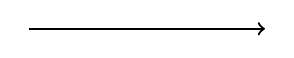
\begin{tikzpicture}
	\draw[thick,->] (0,0) -- (3,0);
	\end{tikzpicture}} \ | \Psi_n \rangle
\end{equation*}
Die Messung ist nicht deterministisch aber die Schröginger-Gleichung ist deterministisch \Huge{\lightning} \normalsize

\section{Einige einfache Quantensysteme}

\begin{itemize}
	\item wir benutzen $ \Psi(\vec{r},t) = \langle \vec{r}|\Psi \rangle $
	\item ein Teilchen der Masse $ m $
	\item eindimensionale Bewergung
	\item nur $ t $-unabhängiger Hamiltonian\\
	$ \Rightarrow $ Zeitunabhängige SGL\\
	$ \Rightarrow $ stationäre Zustände
\end{itemize}
\begin{equation*}
\rmbox{ E \Psi(x) = \left(-\frac{\hbar^2}{2m} \prt{^2}{x^2} + V(x)\right) \Psi(x) }
\end{equation*}
Physikalische Bedingungen an die Lösung:
\begin{enumerate}[(1)]
	\item Anschlussbedingungen an unstetigkeiten.\\
	$ \Psi(x) $ und $ \Psi'(x) $ müssen stetig sein.
	\item Gebundene Teilchen\\
	$ \Rightarrow $ Lösungen müssen normierbar sein\\
	$ \Psi(x \to \pm \infty) = 0 $
\end{enumerate}
\lcom{Die Wellenfunktionen von nicht gebundenen Teilchen sind auch normiert, allerdings ist dies nicht einfach so berechenbar. Eine freie EM-Welle im unendlichen Raum hätte folglich überall winzige Aufenthaltswahrscheinlichkeiten, da wir quasi durch unendlich Teilen. Hierzu müsste man Randbedingungen oder ein endlich großes Universum einführen.}

\subsection{Konstantes Potential \texorpdfstring{$ V(x) = V_0 $}{V(x) = V0}}

Annahme: Teichen läuft von links nach rechts\\
Ansatz: $ \Psi(x) = C e^{i k x} $\\
SGL:
\begin{equation*}
E \Psi = \left(\frac{\hat{\vec{p}}^2}{2m} + \hat{V}_0\right) \Psi
\end{equation*}
$ \hat{V}_0 \Psi = V_0 \Psi \quad V(\hat{\vec{x}}) = V(x) \Psi(x) $\\
Lösung: mit $ \vec{p} = \hbar \vec{k} : $ $ \hbar k = \sqrt{2 m (E - V_0)} $\\
\emph{Bemerkung:}
\begin{itemize}
	\item $ \Psi(x,t) = e^{\frac{i}{\hbar} Et} \Psi(x) + \{ - k \} = C e^{\frac{i}{\hbar} (\hbar k x - Et)} + \{ - k \} $
\end{itemize}

\subsection{Potentialstufe}

\begin{center}
	%t1:
	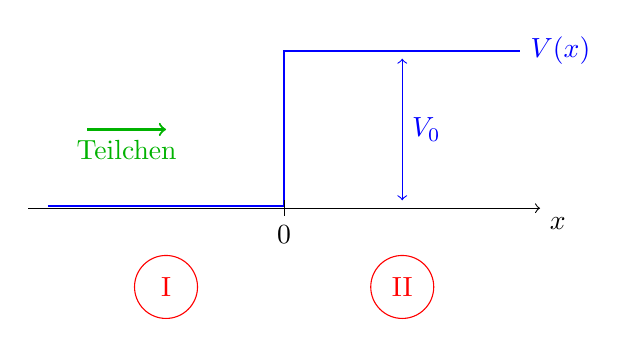
\begin{tikzpicture}
		\draw[thick,blue] (-3,.025) -| (0,2) -- (3,2) node[right] {$ V(x) $};
		\draw[thick,black!30!green,->] (-2.5,1) -- node[below] {Teilchen} ++(1,0);
		\draw[->] (-3.25,0) -- (3.25,0) node[anchor=north west] {$ x $};
		\draw (0,.1) -- ++(0,-.2) node[below] {$ 0 $};
		\node[draw=black,circle, minimum size=.8cm,red] at (-1.5,-1) {I};
		\node[draw=black,circle, minimum size=.8cm,red] at (1.5,-1) {II};
		\draw[<->,blue] (1.5,.1) -- node[right] {$ V_0 $} (1.5,1.9); 
	\end{tikzpicture}
\end{center}
klassisch:
\begin{itemize}
	\item $ E > V_0 : $ Teilchen fliegt weiter aber langsamer
	\item $ E < V_0 : $ Teilchen wird reflektiert (an Wand umkehren)
	$ \Rightarrow $ kann sich \textbf{nicht} im Bereich II aufhalten
\end{itemize}
Quantenmechanik:\\
\folie{Reflektion und Transmission}
\begin{itemize}
	\item $ E > V_0 : $\\
	Lösung in I:
	\begin{equation*}
	\Psi_{I}(x) = e^{i k x} + R e^{- i k x} \qquad \hbar k = \sqrt{2 m E} \quad \
	\end{equation*}
	Lösung in II:
	\begin{equation*}
	\Psi_{II}(x) = T e^{i q x} \qquad \qquad \hbar q = \sqrt{2 m (E - V_0)}
	\end{equation*}
	\lcom{Mit dem neuen Wellenvektor $ q $!}\\
	Anschlussbedingungen: $ \Psi_{I}(0) = \Psi_{II}(0) $ und Ableitungen $ \Psi'_{I}(0) = \Psi'_{II}(0) $
	\lcom{Hier kommen die Stetigkeitsbedingungen aus der Schrödinger-Gleichung statt wie in der Elektodynamik aus den Maxwell-Gleichungn.}
	\begin{equation*}
	\Rightarrow \quad \rmbox{ R = \frac{k - q}{k + q} \qquad T = \frac{2 k}{k + q} }
	\end{equation*}
	physikalische Bedeutung der Lösung:\\
	mit der Wahrscheinlichkeit $ R^2 $ wird die Welle reflektiert \\
	mit der Wahrscheinlichkeit $ T^2 $ wird die Welle transmittiert (läuft weiter)\\[5pt]
	\emph{Bemerkung:}\\
	Wann ist $ R^2 + T^2 \neq 1 $ ?\\
	\lcom{Aufgrund der veränderten Wellenlänge muss mit eingerechnet werden.}\\
	$ 1 - R^2 = \frac{q}{k} T^2 $
	\item $ E < V_0 : $\\
	gleicher Ansatz: aber Wellenvektor im Bereich II ist imaginär
	\begin{equation*}
	\Rightarrow \quad \Psi_{II}(x) = T e^{i q x} \equiv T e^{- \kappa x}
	\end{equation*}
	$ \hbar \kappa \rightarrow - i \hbar q $ bzw. $ \hbar q \rightarrow i \hbar \kappa $\\
	$ \Rightarrow $ Welle im Bereich II fällt exponentiell ab\\
	$ \Rightarrow $ $ q \to i \kappa $
	\begin{equation*}
	\Rightarrow \quad \rmbox{ R = \frac{k - i \kappa}{k + i \kappa} \qquad T = \frac{2 k}{k + i \kappa} }
	\end{equation*}
	$ |R|^2 = 1 $\\
	\folie{Tunnel-Effekt}
\end{itemize}
\textbf{Fall einer unendlich hohen Potentialstufe} $ V_0 \to \infty $\\
$ \Rightarrow \quad \gamma \to \infty $\\
$ \Rightarrow \quad R = - 1 \quad T = 0$\\
$ \Rightarrow \quad \Psi_{\tx{I}}(x) = e^{i k x} - e^{- i k x} $\\
$ \Rightarrow \quad \Psi_{\tx{II}}(x) = 0 $

% Vorlesung 23.01.

\subsection{Potentialbarriere}

\begin{center}
	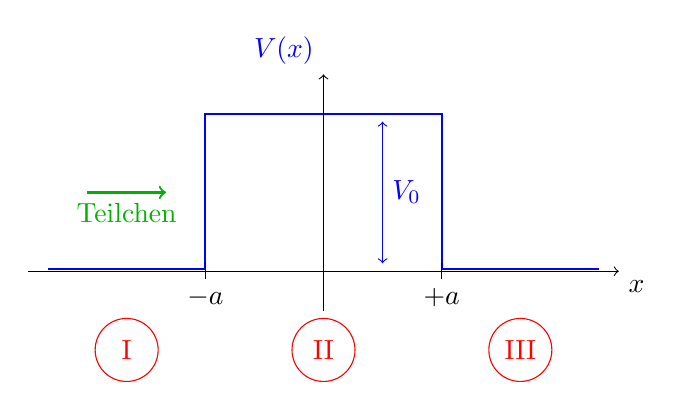
\begin{tikzpicture}
		\draw[thick,blue] (-3.5,.025) -| (-1.5,2) -- (1.5,2) |- (3.5,.025);
		\draw[thick,black!30!green,->] (-3,1) -- node[below] {Teilchen} ++(1,0);
		\draw[->] (-3.75,0) -- (3.75,0) node[anchor=north west] {$ x $};
		\draw[->] (0,-0.5) -- (0,2.5) node[anchor=south east] {\color{blue}$ V(x) $};
		\draw (-1.5,.1) -- ++(0,-.2) node[below] {$ -a $};
		\draw (1.5,.1) -- ++(0,-.2) node[below] {$ +a $};
		\node[draw=black,circle, minimum size=.8cm,red] at (-2.5,-1) {I};
		\node[draw=black,circle, minimum size=.8cm,red] at (0,-1) {II};
		\node[draw=black,circle, minimum size=.8cm,red] at (2.5,-1) {III};
		\draw[<->,blue] (.75,.1) -- node[right] {$ V_0 $} ++(0,1.8); 
	\end{tikzpicture}
\end{center}
\folie{Potentialstufe}\\
klassisch:
\begin{itemize}
	\item $ E > V_0 : $ Teilchen fliegt darüber
	\item $ E < V_0 : $ Teilchen wird am Potential umgekehrt 
\end{itemize}
Quantenmechanik:
\begin{itemize}
	\item Bereich I:
	\begin{equation*}
	\, \Psi_{\tx{I}}(x) = e^{i k x} + R e^{- i k x} \qquad \hbar k = \sqrt{2 m E}
	\end{equation*}
	\item Bereich II:
	\begin{equation*}
	\qquad \qquad \Psi_{\tx{II}}(x) = B e^{i q x} + C e^{- i q x} \qquad \hbar q = \sqrt{2 m (E - V_0)} \
	\end{equation*}
	\item Bereich III:
	\begin{equation*}
	\Psi_{\tx{III}}(x) = T e^{i k x} \hspace{4.4cm}
	\end{equation*}
\end{itemize}
$ + $ Anschlussbedingungen
\begin{itemize}
	\item Fall $ E < V_0 : $ $ \Rightarrow  q $  ist imaginär $ \qquad \hbar \kappa = - i \hbar q $
	\begin{equation*}
	\Rightarrow \qquad \Psi_{\tx{II}}(x) = B e^{- \kappa x} + C e^{\kappa x}
	\end{equation*}
	$ \Rightarrow $ Anschlussbedingungen\\
	\begin{equation*}
	T = \frac{e^{-ikq}}{\cosh (\kappa a) + i \epsilon \sinh (\kappa a)} \qquad \epsilon = \frac{1}{2} \left(\frac{\kappa}{k} - \frac{k}{\kappa}\right)
	\end{equation*}
	\item Fall $ E > V_0 : $ analog dazu
\end{itemize}
\folie{Tunneleffekt}\\
$ \Rightarrow $ \textbf{Tunneleffekt}\\[5pt]
\textbf{Tunnelwahrscheinlichkeit:}
\begin{equation*}
t(E) = T^2 = \left(1 + \frac{V_0^2}{4 E(V_0 - E)} \sinh^2 (\kappa a) \right)^{-1}
\end{equation*}
\lcom{Die Tunnelwahrscheinlichkeit hängt also vor allem von dem Potentialunterschied und der ,,Dicke der Wand`` ab.}
\begin{center}
	% unnumbered tikz *-*:
	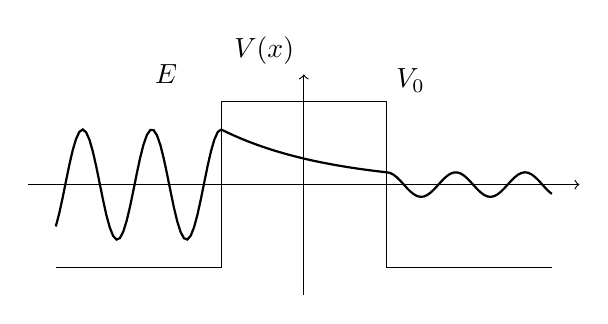
\begin{tikzpicture}[scale=.7]
		\draw (-4.5,-1.5) -| (-1.5,1.5) -- (1.5,1.5) |- (4.5,-1.5);
		\draw[domain=-4.5:-1.5, samples=50, thick] plot (\x, {cos(((\x + 1.5) * 5) r)});
		\draw[domain=-1.5:1.5, samples=50, thick] plot (\x, {exp(-(\x + 1.5) * 0.5)});
		% 0,135335283
		% 0,22313016
		\draw[domain=1.5:4.5, samples=50, thick] plot (\x, {0.22313016 * cos(((\x - 1.5) * 5) r)});
		\draw[->] (-5,0) -- (5,0);
		\draw[->] (0,-2) -- (0,2) node[anchor=south east] {$ V(x) $};
		\node (E) at (-2.5,2) {$ E $};
		\node[anchor=south west] (v) at (1.5,1.5) {$ V_0 $};
	\end{tikzpicture}
\end{center}
\lcom{Die Wahrscheinlichkeit auf der anderen Seite gemessen zu werden ist kleiner aber die Energie ist die selbe \mau}\\[5pt]
\textbf{Diskussion:}
\begin{enumerate}[i)]
	\item $ \kappa a \gg 1 $ (hohe und breite Barriere)
	\begin{equation*}
	\Rightarrow \quad t(E) \cong \tx{exp} \left[- \frac{2 a}{\pi} \sqrt{2 m (V_0 - E)}\right]
	\end{equation*}
	\lcom{Die Tunnelwahrscheinlichkeit wird also exponentiell kleiner mit den Faktoren der Höhe und Breite der Barriere.}
	\item Im Rahmen der WKB-Näherung ergibt sich für allgemeine Potentialbarrieren $ V(x) $
	\begin{equation*}
	\Rightarrow \quad t(E) = \tx{exp} \left[- \frac{2}{\hbar} \int_{a}^{b} \sqrt{2m(V(x) - E)} \dd x\right]
	\end{equation*}
	$ a,b : $ klassische Umkehrpunkte
	\folie{WKB-Näherung}\\
	\lcom{Bei der WKB-Näherung integriert man über verschiedene Potentiale und summiert somit also die exponentiellen Abfälle durch diese infinitesimal dünnen Barrieren.}\\
\end{enumerate}

\subsection{Beispiele für den Tunneleffekt}

\emph{Beispiel:} Zerfallswahrscheinlichkeit
\begin{enumerate}[1)]
	\item $ \dd N = - \frac{N}{\tau} \dd t $\\
	$ \dd N = - N \cdot \tx{ Zerfallswahrscheinlichkeit} \cdot \dd t $
	\item Zerfallswahrscheinlichkeit $ \frac{1}{\tau} = $ Tunnelwahrscheinlichkeit $ \cdot $ Frequenz der Wandstöße\\
	\folie{Tunneln und Zerfallswahrscheinlichkeiten}
	\begin{equation*}
	t_{\alpha}(E) \cong \tx{exp} \left[-\frac{\sqrt{2 m}}{\hbar} \left(\pi e^2 \frac{Z_1 Z_2}{\sqrt{E}} - 4 e \sqrt{Z_1 Z_2}\right)\right]
	\end{equation*}
	$ \Rightarrow $ Kernfusion bevorzugt mit $ Z = $ kleine Kerne\\
	(Alpha-Zerfall ($ \alpha $-Zerfall)) ist die Umkehrreaktion 
\end{enumerate}
\emph{Beispiel:} \textbf{Feldemission}\\[5pt]
\folie{Metall ohne und mit $ \vec{E} $-Feld}\\
thermische Energie $ \gg $ Austrittsarbeit (also keine Glühemission)\\
$ \Rightarrow $ Metall ins starke Feld\\
$ \Rightarrow $ Potentialbarriere
\begin{equation*}
\vec{j}(E) = k_1 \frac{E^2}{W_A} \tx{exp} \left[- \frac{k_2 W_{A}^{\frac{3}{2}}}{|E|}\right]
\end{equation*}
$ k1, k2 : $ für uns hier unwichtige konstanten\\[5pt]
\versuch{Feldemission}
\indent Kathode wird bis zur Glut erhitzt, aber anders als eine Glühwendel, nicht zur Emission von Elektronen sondern zur Reinigung der Nadeloberfläche. An der spitzen Kathode bildet sich bei Anlegung von Spannung ein sehr starkes $ \vec{E} $-Feld. Aufgrund dieser großen Potentialdifferenz können mehr Elektronen Tunneln und werden auf den Leuchtschirm beschleunigt.

Mit einer anderen Konstruktion können wir gezielt Barium Atome in die Glaskugel verdampft. Somit könne wir die Nadelspitze gezielt verunreinigen. Durch diese an der Nadel abgesetzten Atome verringert sich auf kleinen Bereichen der Krümmungsradius und damit der Potentialunterschied. Deshalb erhöht sich an diesen Stellen die Tunnelwahrscheinlichkeit.

Bei sauberer Nadel sieht man, in grün, auf dem Leuchtschirm die Struktur der Nadelspitze (Periodisch aufgrund der Kristallstruktur des Metalls).

Bei gezielter Verunreinigung durch Barium Atome Bilden sich einige (wieder periodisch verteilte) dunkle Flecken mit hellen Rändern (höhere Tunnelwahrscheinlichkeit).

Nun wird die Nadelspitze wieder ein wenig aufgeheizt (nicht genug um sie zu Reinigen). Das Bild wird beweglich und Wabert herum wie heiße Luft. Diese Bewegung ist die Thermische Bewegung der Barium Atome auf der Oberfläche (Brown'sche-Bewegung).\\[10pt]
\emph{Beispiel:} \textbf{kalte Emission}\\[5pt]
$ \rightarrow $ Rastertunnelmikroskop
\begin{equation*}
I(d) \propto \frac{U}{d} \tx{exp} \left[- \frac{2 d}{\hbar} \sqrt{2 m W_A}\right]
\end{equation*}
\folie{Tunneln und Potentiale}\\
\folie{Carbon-Kristallstruktur und Rastertunnelmikrokopaufnahme}\\
genaue Analyse:
\begin{equation*}
I(d) \approx | \Psi_{\tx{Oberfläche}} |^2 e^{- \Lambda d}
\end{equation*}
$ \Rightarrow $ \textbf{Quantenkäfige}\\
\folie{Bilder zu Quantenkäfigen}\\
Aus Interferenz entstehende Wellenfunktion der gefangenen Elektronen ist im Rastertunnelmikroskop gut Sichtbar. Bei Kreisförmigem Käfig: Sehr Wahrscheinlich in der Mitte. Bei Ellipsenförmigem Käfig sehr Wahrscheinlich in einem der beiden Brennpunkte.\\[10pt]
\emph{Beispiel:} \textbf{Tunneldiode}\\[5pt]
\folie{Tunneldiode}\\
Man kann damit einen Spannungsabhängigen negativen Widerstand herstellen.\\[10pt]
\emph{Beispiel:} \textbf{Elektrodynamik}\\[5pt]
\textbf{evaneszente Wellen} \folie{evaneszente Wellen}

\subsection{Harmonischer Oszillator}

$ \Rightarrow V(x) = \frac{1}{2} D x^2 \equiv \frac{m \omega_0^2}{2} x^2 \qquad \omega = \sqrt{\frac{D}{m}} $\\
$ \Rightarrow $ Hamiltonfunktion:
$$ \ham(\vec{p}, \vec{x}) = \frac{\vec{p}^2}{2m} + \frac{1}{2} D \vec{x}^2 $$
$ \Rightarrow $ Hamiltonoperator:\\
zeitunabhängige SGL
\begin{equation*}
\rmbox{ E \Psi(x) = \left(-\frac{\hbar^2}{2m} \prt{^2}{x^2} + \frac{m \omega_0^2}{2} x^2\right) \Psi(x) }
\end{equation*}
klassisch:
\begin{itemize}
	\item $ E = 0 : $ Teilchen ist in Ruhe bei $ x = 0 $
	\item $ E > 0 : $ Teilchen schwingt mit Amplitude $ A $
	\begin{equation*}
	E = \frac{1}{2} m \omega_0^2 A^2
	\end{equation*}
	Die Aufenthaltswahrscheinlichkeit am Ort $ x $\\
	(im Bereich von $ a $ bis $ b $)
	\begin{equation*}
	p(t) \dd t = \frac{1}{T} \dd t = p(x) \dd x
	\end{equation*}
	\begin{equation*}
	\Rightarrow \quad p(x) = \left(2 \pi A \sqrt{1 - \left(\frac{x}{A}\right)^2}\right)^{-1} = \frac{\omega_0}{2 \pi V(x)}
	\end{equation*}
\end{itemize}
Quantenmechanisch:\\[5pt]
Die SGL kann für den harmonischen Oszillator exakt gelöst werden\\
Zusammenhang mit den sog. Hermitpolynomen $ H_{n}(x) = (-1)^n e^{x^2} \frac{d^n}{a x^n} e^{-x^2} \quad n \in \mathbb{N}_0 $\\[5pt]
Energie:
$$ E_n = \hbar \omega_0 \left(n + \frac{1}{2}\right) \quad n \in \mathbb{N}_0 $$
Grundzustand:
$$ \Psi_0(x) = \frac{1}{\sqrt{\sqrt{\pi} x_0}} e^{-\frac{1}{2} \left(\frac{x}{x_0}\right)^2} \qquad x_0 = \sqrt{\frac{\hbar}{m \omega_0}} $$
Anregungszustände:
\begin{equation*}
\Psi_{m > 0} (x) = \frac{1}{\sqrt{2^n n! \sqrt{\pi} x_0}} H_n \left(\frac{x}{x_0}\right) e^{-\frac{1}{2} \left(\frac{x}{x_0}\right)^2}
\end{equation*}

% Vorlesung 29.01

%Wiederholugn der letzten Vorlesung (Energie Grunszustand Anregungszustände)

\noindent
\textbf{Definition:} Erwartungswert eines Operators
\begin{equation*}
\langle \hat{O} \rangle_n = \langle \Psi_n | \hat{O} | \Psi_n \rangle = \int \Psi^*_n(x) \hat{O} \Psi_n(x) \ \dd x
\end{equation*}
Erwartungswerte
\begin{align*}
\langle \hat{x} \rangle_n &= 0\\
\langle \hat{p} \rangle_n &= 0\\
\langle \hat{x}^2 \rangle_n &= x_0^2 \left(n + \frac{1}{2}\right)\\
\langle \hat{p}^2 \rangle_n &= \frac{\hbar^2}{x_0^2} \left(n + \frac{1}{2}\right)
\end{align*}
\folie{Wellenfunktionen und Potentiale}

\subsection{Beispiele für den quantenmechanischen Oszillator (QHO)}

\emph{Beispiel:} Schwingungszustände in mehratomigen Molekülen und Festkörpern\\
\folie{Molekülschwingungen und Bindungspotential der Atomen im Molekül oder Festkörper}\\
\folie{Federmodel für Molekül und Festkörperschwingungen}\\
\lcom{Wo sieht man diese Schwingungen? Zum Beispiel wenn wir Schall durch einen Festkörper jagen bewegen sich die Kerne (nicht die elektronen) in dieser Harmonischen schwingungn mit und klingen dann in ihren Eigenfrequenzen (siehe Stimmgabel).}\\[5pt]
\emph{Beispiel:} EM-Strahlung
\begin{equation*}
E_n = \hbar \omega_0 n \qquad \tx{Planck}
\end{equation*}
\vspace{3pt}
\begin{equation*}
% t1:
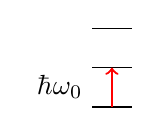
\begin{tikzpicture}[scale=.5]
	\foreach \y in {0, 1, 2}
	\draw (0,\y) -- ++(1,0);
	\node[left] at (0,.5) {$ \hbar \omega_0 $};
	\draw[thick,red,->] (.5,0) -- (.5,1);
\end{tikzpicture}
\qquad 
\begin{array}{c}
\tx{\color{red} Photon \color{black} $ \quad $ Einstein}\\[5pt]
\phantom{0}
\end{array}
\end{equation*}

\subsection{Unschärferelation und Quanten- klassischer Übergang}

\textbf{Definition:} Schwankung/Unschärfe
\begin{equation*}
\left(\Delta O\right)^2 = \left\langle \left(\hat{O} - \langle \hat{O} \rangle ^2\right) \right\rangle = \langle \hat{O}^2 \rangle - \langle \hat{O} \rangle^2
\end{equation*}
\emph{Bemerkung:}
\begin{equation*}
\langle \hat{O}^n \rangle = \int \Psi* \hat{O}^2 \Psi \ \dd x
\end{equation*}

\subsubsection{Nullpunktschwingung}

Grundzustand $ E_0 = \frac{1}{2} \hbar \omega_0 $
\begin{equation*}
\Rightarrow \quad \tx{Der QM Oszillator kann \textbf{NICHT} zur Ruhe kommen}
\end{equation*}
\lcom{Anders als ein Pendel, das KANN man einfach anhalten \mau}
\begin{align*}
\Delta x^2 &\equiv \langle \hat{x}^2 \rangle = x_0^2 \left(n + \frac{1}{2}\right) \overset{n = 0}{\longrightarrow} \frac{1}{2} x_0^2\\
\Delta p^2 &\equiv \langle \hat{p}^2 \rangle = \frac{\hbar^2}{x_0^2} \left(n + \frac{1}{2}\right) \overset{n = 0}{\longrightarrow} \frac{\hbar^2}{2 x_0^2}
\end{align*}

\subsubsection{Unschärferelation}

Pärchen von Operatoren $ \hat{A}, \hat{B} $
\begin{equation*}
\left[\hat{A}, \hat{B}\right] \defeq \hat{A} \hat{B} - \hat{B} \hat{A} = \casess{0}{\tx{komutieren}}{\neq 0}{\tx{komutieren nicht}}
\end{equation*}
\begin{equation*}
\left[\hat{A}, \hat{B}\right] \Psi = \hat{A} \hat{B} \Psi - \hat{B} \hat{A} \Psi = \casess{= 0}{\tx{komutieren}}{\neq 0}{\tx{komutieren nicht}}
\end{equation*}
\begin{equation*}
\Rightarrow \quad \Delta A \cdot \Delta B \ge \frac{1}{2} \left|\left\langle \left[\hat{A}, \hat{B}\right] \right\rangle\right|
\end{equation*}
z.B. der Orts- und Impulsoperator
\begin{equation*}
\left[\hat{x}, \hat{p}\right] = i \hbar
\end{equation*}
\begin{equation*}
\Rightarrow \quad \rmbox{\Delta x \Delta p \ge \frac{1}{2} \hbar}
\end{equation*}
$ \Rightarrow $ QHO:
\begin{equation*}
\Delta x \Delta p = \hbar \left(n + \frac{1}{2}\right) \overset{n = 0}{\longrightarrow} \frac{1}{2} \hbar
\end{equation*}
\lcom{Der QHM hat die Unschärferelation also so gut wie möglich ausgenutzt \mau}
\begin{equation*}
\Rightarrow \quad \tx{Nullpunktschwingung ist eine Konsequenz der Unschärfereltaion \mau}
\end{equation*}

\subsubsection{Quanten- klassischer Übergang}

Aufenthaltswahrscheinlichkeit:\\
\begin{minipage}{.5\linewidth}
	klassisch:
	\begin{equation*}
	p(x) = \frac{\omega_0}{2 \pi V(x)}
	\end{equation*}
\end{minipage}%
\begin{minipage}{.5\linewidth}
	Quantenmechanik:
	\begin{equation*}
	\left|\Psi_n(x)\right|^2
	\end{equation*}
\end{minipage}%
\\
\folie{Wellenfunktion und Aufenthaltswahrscheinlichkeit}\\
für größere $ n $ nähern sich $ p(x) $ und $ \left|\Psi_n(x)\right|^2 $ an.\\[5pt]
$ \Rightarrow \quad $ je größer der Oszillator angeregt ist, um so klassischer wird er \mau\\[5pt]
,,Amplitude`` der Schwingung\\
\lcom{Das Wort Amplitude ist hier mit Vorsicht zu behandeln, da wir hier die Zeitunabhängige SGL betrachtet haben \mau Deshalb erhalten wir auch keine Schwingenden Erwartungswerte: Die Erwartungswerte von Stationären Zustände sind ebenfalls Stationär. Es geht hier also um Aufenthaltswahrscheinlichkeiten und nicht um das Tatsächliche verfolgen eines Schwingenden Objekts (Es gibt solche zeitabhängigen, schwingenden Zustände, diese sind jedoch komplizierter und werden in den folgenden Vorlesungen Behandelt).}\\[5pt]
Varianz: $ \Delta x^2 \equiv \langle \hat{x^2} \rangle - \langle \hat{x} \rangle^2 \propto A^2 $
\begin{center}
	\begin{tabular}{l|l|l}
		& klassisch & Quantenmechanik\\
		\hline
		& & \\[-5pt]
		%
		Energie & $ E = \frac{1}{2} m \omega_0^2 A^2 = \hbar \omega_0 \frac{m \omega_0}{2 \hbar} A^2 $ & $ E_n = \hbar \omega_0 \left(n + \frac{1}{2}\right) $\\[7pt]
		\hline
		& & \\[-5pt]
		Schwingung & $ \Delta x^2 = \langle x^2 \rangle = \frac{1}{2} A^2 $ & $ \Delta x^2 = \langle \hat{x^2} \rangle = x_0^2 \left(n + \frac{1}{2}\right) $\\[7pt]
	\end{tabular}
\end{center}
\begin{equation*}
\frac{1}{2} A^2 \quad \longleftrightarrow \quad x_0^2 \left(n + \frac{1}{2}\right)
\end{equation*}
$ \Rightarrow $ je höher der Oszillator angeregt ist, desto größer ist seine ,,Amplitude``
\begin{center}
	% t2:
	\begin{tikzpicture}
		\node (1) at (0,0) {$ \substack{\tx{\normalsize höher} \\ \tx{\normalsize angeregt}} $};
		\node (2) at (0,-2.5) {,,A`` größer};
		\node (3) at (3.5,0) {$ \substack{\tx{\normalsize Energie} \\ \tx{\normalsize höher}} $};
		\node (4) at ($ (2) + (3) $) {klassischer};
		\foreach \a\b in {1/2,1/3,2/4,3/4,1/4,2/3}
		\draw[line width=1.1,<->] (\a) -- (\b);
	\end{tikzpicture}
\end{center}
\lcom{Zur Unschärferelation: statistische Mechanik: bei häufigem Würfeln geht die Schwankung nicht gegen 0 sonder fehlt mit $ \sqrt{n} $ ab. Der relative Fehler ist somit mit $ \frac{\sqrt{n}}{n} $ gegeben. Der Messwert wird also trotz steigendem Fehler immer Genauer. In der Quantenmechanik können wir z.B. den QHM sehr hoch anregen (hohes $ n $) und damit $ \Delta x $ und auch $ \Delta p $ sehr scharf festlegen. Hier sieht man wieder bei einer hohen Anregung (Quanten- klassischer Übergang), dass die Unschärferelation weniger gut gilt und man wieder von scharfem Impuls und Ort reden (gleichzeitig Messbar, anders als in der QM).}

\section{Elektron im Coulomb-Feld einer Zentralladung}

Elektron: $ q = -e $\\
positive Zentralladung $ Q = + Z e $\\[5pt]
Coulomb-Potential
\begin{equation*}
V(\vec{r}) = - \frac{Ze^2}{4 \pi \epsilon r}
\end{equation*}
\lcom{Alles was mit Planetenbahnen zu tun hat wir im Folgenden als bekannt vorrausgesetzt.\\
Lenz'scher Vektor: konstante die geschlossene Ellipsenbahnen begründet. Mit Relativistischen Effekten, wie bei Merkur, ergeben sich Rosettenbahnen.}\\[5pt]

\subsubsection{Zeitunabhängige SGL (Ortsdarstellung)}

\begin{equation*}
E \Psi(\vec{r}) = \left[- \frac{\hbar^2}{2m} \left(\prd{^2}{x^2} + \prd{^2}{y^2} + \prd{^2}{z^2}\right) - \frac{Z e^2}{4 \pi \epsilon_0 r}\right] \Psi (\vec{r})
\end{equation*}
\lcom{Dies genügt hier, da wir und wie bei der Planetenbewegung auf den Massenmittelpunkt beziehen, d.h. alle anderen Abstände gelten relativ zwischen den beiden Körpern.}

\subsubsection{Wichtige Eigenschaften}

\begin{enumerate}[(1)]
	\item 3-dimensionales Problem
	\item hat eine hohe Symmetrie
	\begin{itemize}
		\item Coulomb Potential $ \rightarrow $ 
		\item hat den spezielle $ \frac{1}{r} $ Verlauf
	\end{itemize}
\end{enumerate}
$ \Rightarrow \quad $ siehe Kepler-Problem

\subsubsection{Ideen zur Lösung der SGL}

\lcom{Dies wird eigentlich zu kompliziert und involviert Mathematik, die wir noch nicht beherrschen.\\
Im folgenden die grobe Idee:}
\begin{enumerate}[(1)]
	\item Einschränkung der Lösung auf gebundene Zustände
	$ E < 0 : $\\
	$ \Rightarrow $ Normierbarkeit der Wellenfunktionen
	\begin{equation*}
	\lim\limits_{r \to \infty} \left|\Psi(\vec{r})\right|^2 \to 0
	\end{equation*}
	muss gegeben sein (es muss nicht nur gegen 0 gehen sondern auch schnell genug abfallen!)
	\item Zentralsymmetrisches Problem $ \rightarrow $ Kugelkoordinaten $ r, \theta, \varphi $
	\begin{equation*}
	\vec{r} = r \begin{pmatrix}
	\cos \varphi \sin \theta \\ \sin \varphi \sin\theta \\ \cos \theta
	\end{pmatrix}
	\end{equation*}
	\item Separationsansatz für die Wellenfunktion
	\begin{equation*}
	\Rightarrow \quad \Psi(r,\theta,\varphi) = R(r) \mathcal{Y}(\theta,\varphi)
	\end{equation*}
\end{enumerate}
\emph{Bemerkung:}\\
\lcom{Kugelkoordinaten: wenn wir Kugelkoordinaten wählen machen wir eine implizite Wahl. Somit brechen wir die Symmetrie. Wir müssen nun also Rechnen (Koordinatentransformation) um die Kugelsymmetrie wieder Sichtbar zu machen.\\
Ein Problem, dass sich hier ergibt ist, dass wir eine $ z $-Achse wählen und $ \theta $ und $ \varphi $ davon abhängig machen. Somit werden die Ergebnisse in jedem Fall Rotationssymmetrisch. Für eine gut sichtbare Kugelsymmetrie muss noch weiter gerechnet werden. Diese $ z $-Achse nennt man in der Quantenmechanik die Quantisierungsachse.}
%\begin{itemize}
%	\item 
%\end{itemize}

% Vorlesung 30.01.

\subsection{Lösung der SGL}

5 Schritte
\begin{enumerate}[(1)]
	\item Transformation auf Kugelkoordinaten $ \vec{r} \to r, \theta, \varphi $
	\begin{equation*}
	\Rightarrow \quad \prd{^2}{x^2} + \prd{^2}{y^2} + \prd{^2}{z^2} \to \frac{1}{r^2} \prt{}{r} \left(r^2 \prt{}{r}\right) + \frac{1}{r^2 \sin \theta} \prt{}{\theta} \left(\sin \theta \prt{}{\theta}\right) + \frac{1}{r^2 \sin^2 \theta} \prt{^2}{\varphi^2}
	\end{equation*}
	%
	% make me smaller or a bit bigger:
	%
	\begin{footnotesize}
		\begin{equation*}
		\Rightarrow \quad E \Psi(r,\theta,\varphi) = \left[-\frac{\hbar^2}{2m} \left(\frac{1}{r^2} \prt{}{r} \left(r^2 \prt{}{r}\right) + \frac{1}{r^2 \sin \theta} \prt{}{\theta} \left(\sin \theta \prt{}{\theta}\right) + \frac{1}{r^2 \sin^2 \theta} \prt{^2}{\varphi^2}\right) - \frac{Ze^2}{4 \pi \epsilon r} \right] \Psi(r,\theta,\varphi)
		\end{equation*}
	\end{footnotesize}
	\emph{Bemerkung}
	\begin{itemize}
		\item $ x(r,\theta,\varphi), y(r,\theta,\varphi), z(r,\theta,\varphi) $
	\end{itemize}
	\item Vereinfachung mit Drehimpuls
	\begin{equation*}
	\tx{klassisch: } \quad \vec{L} = \vec{r} \times \vec{p} \qquad \tx{QM: } \quad \hat{\vec{L}} = \hat{\vec{r}} \times \hat{\vec{p}}
	\end{equation*}
	\begin{equation*}
	\Rightarrow \quad \hat{\vec{p}}^2 = - \hbar^2 \frac{1}{r^2} \prt{}{r} \left(r^2 \prt{}{r}\right) + \frac{1}{r^2} \hat{\vec{L}}^2
	\end{equation*}
	\begin{equation*}
	\Rightarrow \quad E \Psi(r,\theta,\varphi) = \left[-\frac{\hbar^2}{2mr^2} \prt{}{r} \left(r^2 \prt{}{r}\right) + \ub{\frac{\hat{\vec{L}}^2}{2mr^2} - \frac{Ze^2}{4 \pi \epsilon_0 r}}_{\mathclap{\tx{effektieves Potential}}}\right] \Psi(r,\theta,\varphi)
	\end{equation*}
	Das Effektive Potential berechnet sich aus der Fliehkraft minus der Coulomb Kraft.
	\item Seperation in $ R(r) $ und $ \mathcal{Y}(\theta,\varphi) $\\
	Der Hamiltonoperator hat diese Struktur:
	\begin{equation*}
	\hat{\ham} = \hat{\ham}_{R}(r) + f(r) \hat{\ham}_{\mathcal{Y}}(\hat{\vec{L}})
	\end{equation*}
	\begin{equation*}
	\Rightarrow \quad \Psi(r,\theta,\varphi) = R(r) \mathcal{Y}(\theta,\varphi)
	\end{equation*}
	\begin{align*}
	\Rightarrow \tx{Gl. \#1} & \quad \hat{\vec{L}}^2 \mathcal{Y}(\theta,\varphi) = \color{red} c \color{black} \ \mathcal{Y}(\theta,\varphi) \label{1} \tag{\#1}\\
	\tx{Gl. \#2} & \quad \left[-\frac{\hbar^2}{2m} \prt{}{r} \left(r^2 \prt{}{r}\right) + \frac{\color{red} c \color{black}}{2 m r^2} - \frac{Ze^2}{4 \pi \epsilon_0 r}\right] R(r) = E R(r) \label{2} \tag{\#2}
	\end{align*}
	\lcom{Das c ist eine Konstante die aus dem Seperationsansatz kommt. Genau wie das E bei der Herleitung zur Zeitunabhängigen SGL.}\\[5pt]
	\emph{Bemerkung:}
	\begin{equation*}
	E R(r) \mathcal{Y}(\theta,\varphi) = \left[\hat{\ham}_{R}(r) + f(r) \hat{\ham}_{\mathcal{Y}}(\hat{\vec{L}})\right] R(r) \mathcal{Y}(\theta,\varphi)
	\end{equation*}
	\begin{equation*}
	\left[E - \hat{\ham}_{R}(r)\right] R(r) \mathcal{Y}(\theta,\varphi) = f(r) \hat{\ham}_{\mathcal{Y}}(\hat{\vec{L}}) R(r) \mathcal{Y}(\theta,\varphi) = f(r) R(r) \hat{\ham}_{\mathcal{Y}}(\hat{\vec{L}}) \mathcal{Y}(\theta,\varphi)
	\end{equation*}
	\begin{equation*}
	\Rightarrow \quad \frac{\left[E - \hat{\ham}_{R}(r)\right] R(r)}{f(r) R(r)} = c = \frac{\hat{\ham}_{\mathcal{Y}}(\hat{\vec{L}}) \mathcal{Y}(\theta,\varphi)}{\mathcal{(\theta,\varphi)}}
	\end{equation*}
	\begin{align*}
	\Rightarrow \quad \tx{\# 1: } & \quad \hat{\ham}_{\mathcal{Y}}(\hat{\vec{L}}) \mathcal{Y}(\theta,\varphi) = c \mathcal{Y}(\theta,\varphi) \\
	\tx{\# 2: } &  \quad \left[E - \hat{\ham}_{R}(r)\right] R(r) = c f(r) R(r)
	\end{align*}
	\begin{flushright}
		$ \square $
	\end{flushright}
	\item Lösung von Gleichung \eqref{1}\\[5pt]
	Drehimpuls Eingenwertgleichung\\
	$ \Rightarrow $ Lösungen sind die Kugelflächenfunktionen $ \mathcal{Y}_{lm}(\theta,\varphi) $
	\begin{equation*}
	\hat{\vec{L}}^2 \mathcal{Y}(\theta,\varphi) = c \mathcal{Y} (\theta,\varphi)
	\end{equation*}
	\begin{equation*}
	\Rightarrow \quad \rmbox{\hat{\vec{L}}^2 \mathcal{Y}_{lm}(\theta,\varphi) = \hbar^2 l(l+1) \mathcal{Y}_{lm}(\theta,\varphi)}
	\end{equation*}
	\begin{equation*}
	\mathcal{Y}_{lm}(\theta,\varphi) = C_{lm} P_{lm} (\cos \theta) e^{i m \varphi} \qquad l \in \mathbb{N}_0 \quad |m| \le l
	\end{equation*}
	\begin{align*}
	\Rightarrow \quad l = 0 & \to m = 0\\
	l = 1 & \to m = -1, 0, 1\\
	l=2 & \to m = -2, -1, 0, 1, 2 \qquad \qquad (2l + 1) \ m \tx{-Werte pro } l
	\end{align*}
	\folie{Kugelflächenfunktionen für verschiedene $ l, m $}\\[5pt]
	\emph{Bemerkungen:}
	\begin{itemize}
		\item $ \mathcal{Y}(\theta,\varphi) $ lassen sich in Polynome von $ x, y, z $ umschreiben
		\begin{align*}
		\mathcal{Y}_{0,0} &\propto 1\\
		\mathcal{Y}_{1,0} &\propto z\\
		\mathcal{Y}_{1,1} &\propto x + i y\\
		\mathcal{Y}_{1,-1} &\propto x - i y\\
		\mathcal{Y}_{2,0} &\propto (ez^2 - 1)
		\end{align*}
		\begin{equation*}
		\tx{Die Ordnung des Polynoms ist gegeben durch } l
		\end{equation*}
		\item Kugelflächenfunktionen $ \rightarrow $ \textbf{Orbitale}
		\begin{equation*}
		\tx{Orbital } \widehat{=} \ |\mathcal{Y}_{l,m} \pm \mathcal{Y}_{l,-m}|
		\end{equation*}
		\begin{align*}
		&s \tx{-Orbital: } l = 0 : \qquad \quad \mathcal{Y}_{0,0} \propto 1\\
		&p_x \tx{- } \qquad \qquad \qquad \qquad \quad p_x \propto \mathcal{Y}_{1,1} + \mathcal{Y}_{1,-1} \propto x\\
		&p_y \tx{-Orbitale: } l = 1 :  \qquad \, p_y \propto \mathcal{Y}_{1,1} - \mathcal{Y}_{1,-1} \propto y\\
		&p_z \tx{- } \qquad \qquad \qquad \qquad \quad p_z \propto \mathcal{Y}_{1,0} \propto z
		\end{align*}
		% already in align:
		%$ s $-Orbital: $ l = 0 : \qquad \mathcal{Y}_{0,0} \propto 1 $\\
		%$ p_x \qquad \qquad \qquad p_x \propto \mathcal{Y}_{1,1} + \mathcal{Y}_{1,-1} \propto x $\\
		%$ p_y $-Orbitale: $ l = 1 : \qquad \mathcal{Y}_{1,1} - \mathcal{Y}_{1,-1} \propto y $\\
		%$ p_z \qquad \qquad \qquad p_z \propto \mathcal{Y}_{1,0} \propto z $
		\item Notation:
		\begin{equation*}
		l = \qquad 0 \qquad 1 \qquad 2 \qquad 3 \qquad 4 \qquad 5 \qquad 6
		\end{equation*}
		\begin{equation*}
		\qquad \qquad s \qquad p \qquad d \qquad f \qquad g \qquad h \qquad k \
		\end{equation*}
		\folie{Orbitale}
		\item $ \hat{\vec{L}}^2 $ Eingenwertgleichung $ \quad \Rightarrow \quad $ Eingenwert $ l(l+1) $\\[5pt]
		$ \Rightarrow $ Länge des Drehimpulses $ \widehat{=} \ \sqrt{l(l+1)} $\\
		\lcom{In der QM spricht man von Drehimpulsen $ 1, 2, 3 \dots $ also den jeweiligen $ l $-Werten der Orbitale.}\\[5pt]
		$ \hat{L}_z $ Eigenwertgleichung $ \quad \Rightarrow \quad $ Eigenwert $ m $:
		\begin{equation*}
		\hat{L}_z \mathcal{Y}_{lm}(\theta,\varphi) = \hbar m \mathcal{Y}_{lm}(\theta,\varphi)
		\end{equation*}
		$ \Rightarrow $ Komponente entlang $ z \ \widehat{=} \ m $
	\end{itemize}
	\item Lösung von Gleichung \eqref{2}
	\begin{equation*}
	\Rightarrow \quad c = \hbar^2 l(l+1)
	\end{equation*}
	\begin{equation*}
	\Rightarrow \quad \left[-\frac{\hbar^2}{2mr^2} \prt{}{r} \left(r^2 \prt{}{r}\right) + \frac{\hbar^2 l(l+1)}{2mr^2} - \frac{Ze^2}{4 \pi \epsilon_0 r}\right] R_{ml} (r) = E_n R_{ml} (r)
	\end{equation*}
	\lcom{Warum hängt die Energie $ E_n $ nicht von $ l $ ab. Das hat mit der Kugelsymmetrie und der Drehimpulserhaltung zu tun \mau \ Hier taucht also zum ersten mal auf warum wir Kugelkoordinaten und Drehimpuls benutzen.}
	\begin{equation*}
	\Rightarrow \quad R_{ml}(r) = \tilde{r}^l e^{-\tilde{r}} L_{ml}(2 \tilde{r}) \qquad \tilde{r} = \frac{Z}{n a_B} r
	\end{equation*}
	$ L_{ml} : $ Lagere Polynome\\
	$ a_B : $ Bohr'scher Atomradius $ \approx 0{,}5 \AA $\\[5pt]
	$ n = l+1, l+2, l+3, \dots $
	\begin{equation*}
	\rmbox{E_n = - R_{\mathcal{Y}} \frac{Z^2}{n^2}}
	\end{equation*}
	$ R_{\mathcal{Y}} : $ \textbf{Rydberg Konstante}: $ 13{,}6 \, \tx{eV} $\\
	\folie{Radialfunktionen}\\[5pt]
	Grundzustand: $ n=1, l=0 \qquad E_0 = - R_{\mathcal{Y}} Z^2 $\\
	\lcom{Da die Radialfunktionen exponentiell abfallen (gebundene Zustände) wodurch sie normierbar sind, wie wir es gefordert haben.}\\[5pt]
	erster Angeregter Zustand:
	$ n = 2, \quad \left. \begin{array}{ccc}
	l=0 & s & \ \ \: m=0 \\
	l=1 & p & \left\{ \begin{array}{c}
	\phantom{-}m=-1\\
	m=0\\
	m=1
	\end{array} \right.
	\end{array} \right\} \ \ \substack{\tx{4 Zustände} \\ \tx{energetisch} \\ \tx{entartet}} $\\[5pt]
	zweiter angeregter Zustand
	$ n = 3 \left. \right\} \ \ \left. \begin{array}{ccl}
	l=0 & s & m=0 \\
	l=1 & p & m=-1,0,1 \\
	l=2 & d & m=-2,-1,0,1,2
	\end{array} \right\} \ \ \substack{\tx{9 Zustände} \\ \tx{entartet}} $
\end{enumerate}